\chapter{Solver Parameter Testing}
\label{solvtestchap}

% TODO[X] move preface and rhoreactingfoam stuff into OF det modeling section

% TODO[X] start with setup of rrcf and move Sod into previous 

% TODO[X] 4.3 basically consumes this chapter 

%\section{Preface}

%This chapter will go through progression of research on efficacy for the different solvers and detonation modeling techniques performed during the duration of this thesis work. In an effort to assist the University of Colorado's Turbulence and Energy Systems Laboratory (TESLa), several solvers and methods will be tested for potential for detonation modeling, stability, and accuracy, typically in that order. Additional focus will be on the effects of AMR on the results. 


Now that \verb|rhoReactingCentralFoam| has been selected for use, the solver can be tested further to determine how different selections in solver parameters alter the solution. Parameters that were tested are the Arrhenius equations's pre-exponential factor exponent, the Courant number and time step variation, static mesh resolution, and adaptive mesh refinement variation. Sensitivities to certain solver parameters as well as mesh resolution on the solution were be explored. 


%\section{Solver Parameter Testing and Sensitivity}
Line plots seen in the upcoming sections were sampled with the OpenFOAM utility \verb|postProcess| with the \verb|lineUniform| type, using 1000 sampling points interpolated from cell centers. The line progresses from the edge of the initiation of the detonation to the end of the detonation tube. 

\section{Ignition Tests}
\label{sec:igstudy}

\subsection{Block Ignition}

The block ignition method with high pressure and temperature stoichiometric reactants was utilized initially to build off the work done in \cite{towery1}. A rectangular region spanning from the ignition wall (y-z plane at \(x = 0\) m) to \(x = 0.001\) m was set with a different initial condition than the rest of the domain using the \verb|setFields| utility. The ignition block region contained high pressure and temperature gas at 3000 K and 20 atm, with the rest of the domain at 300 K and 1 atm. This method is seen in Figure \ref{fig:blockig}.
\begin{figure}[h]
\centering
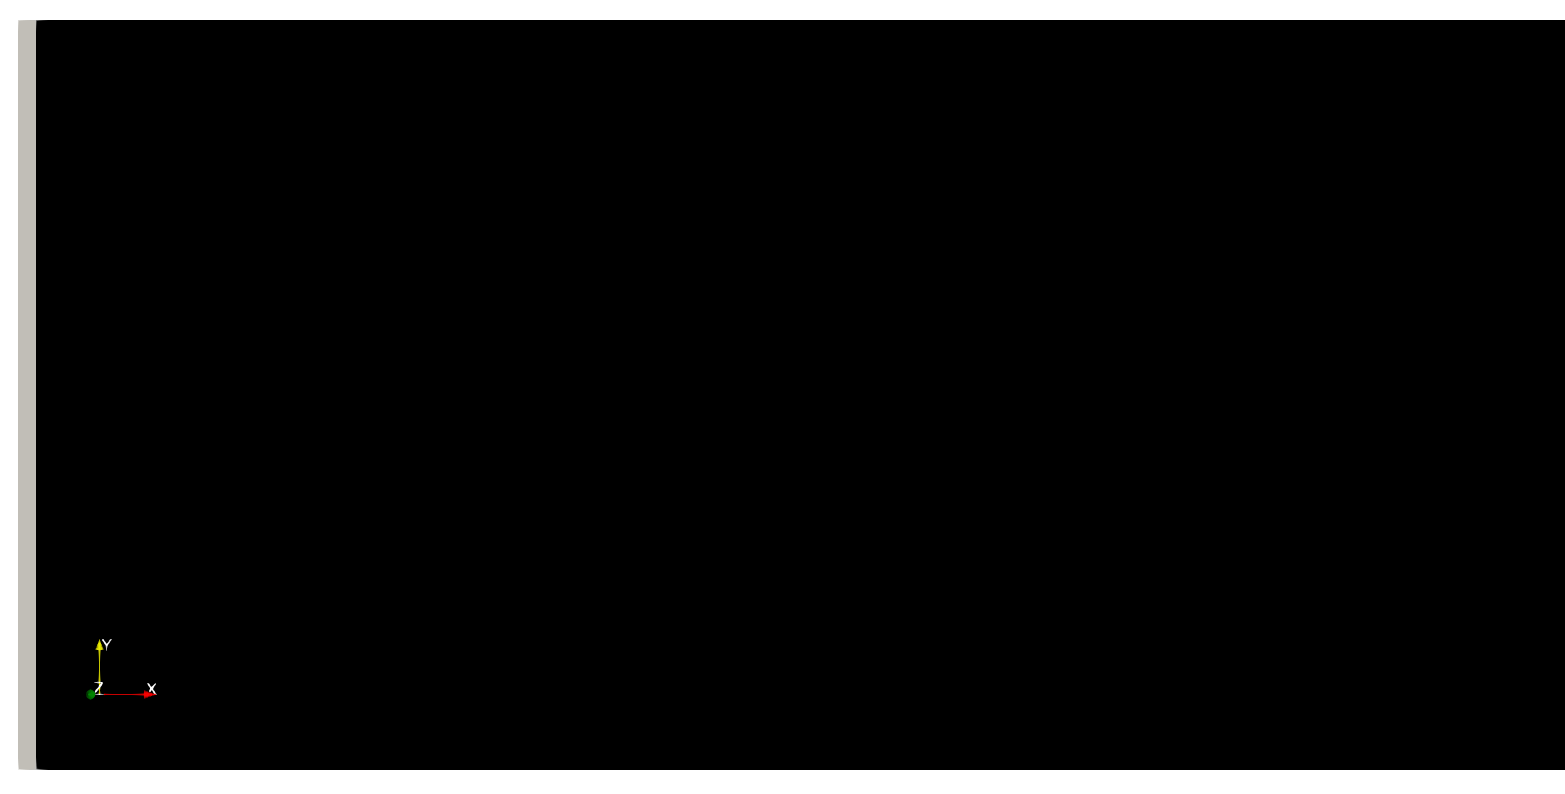
\includegraphics[width=0.8\textwidth]{figs/ignition/block.png}
\caption{Block ignition method, seen on left side of domain, at t = 0 s}
\label{fig:blockig}
\end{figure}%
\noindent Ultimately this ignition approach was not pursued further due to instability in detonation initiation due to the very large gradient in conditions between the block ignition region and the rest of the domain. For both very high and very low grid resolutions, detonation would sometimes not occur and instead the shockwave would decouple from the flame reaction front. A better approach shown by Towery\cite{towery2} is to use a pressure and temperature gradient ranging from the wall to the domain, smoothly transitioning the ignition region to the domain. 

\subsection{Gradient Ignition}
Using the theory shown in Towery\cite{towery2}, we developed an initial gradient ignition condition to guarantee a detonation across mesh resolutions. This gradient ignition spanned 0.01 m from the leftmost wall, ranging from 1200 K at the wall to the domain temperature of 300 K. This can be seen in Figure \ref{fig:gradig}. 
\begin{figure}[h]
\centering
\includegraphics[width=0.8\textwidth]{figs/ignition/gradient.png}
\caption{Gradient ignition method, seen on left side of domain, at t = 0 s}
\label{fig:gradig}
\end{figure}%
\noindent After transitioning to this ignition method, detonations were less noisy and more consistent in their ignition. The next stage towards matching experimental results and other computational detonation modeling was to attempt to model detonation cells. In order to better match experimental conditions and form detonation cells, the temperature gradient initial condition was also expanded to include a randomized 240 K temperature increase throughout the domain seen in Figure \ref{fig:gradrand}.
\begin{figure}[h]
\centering
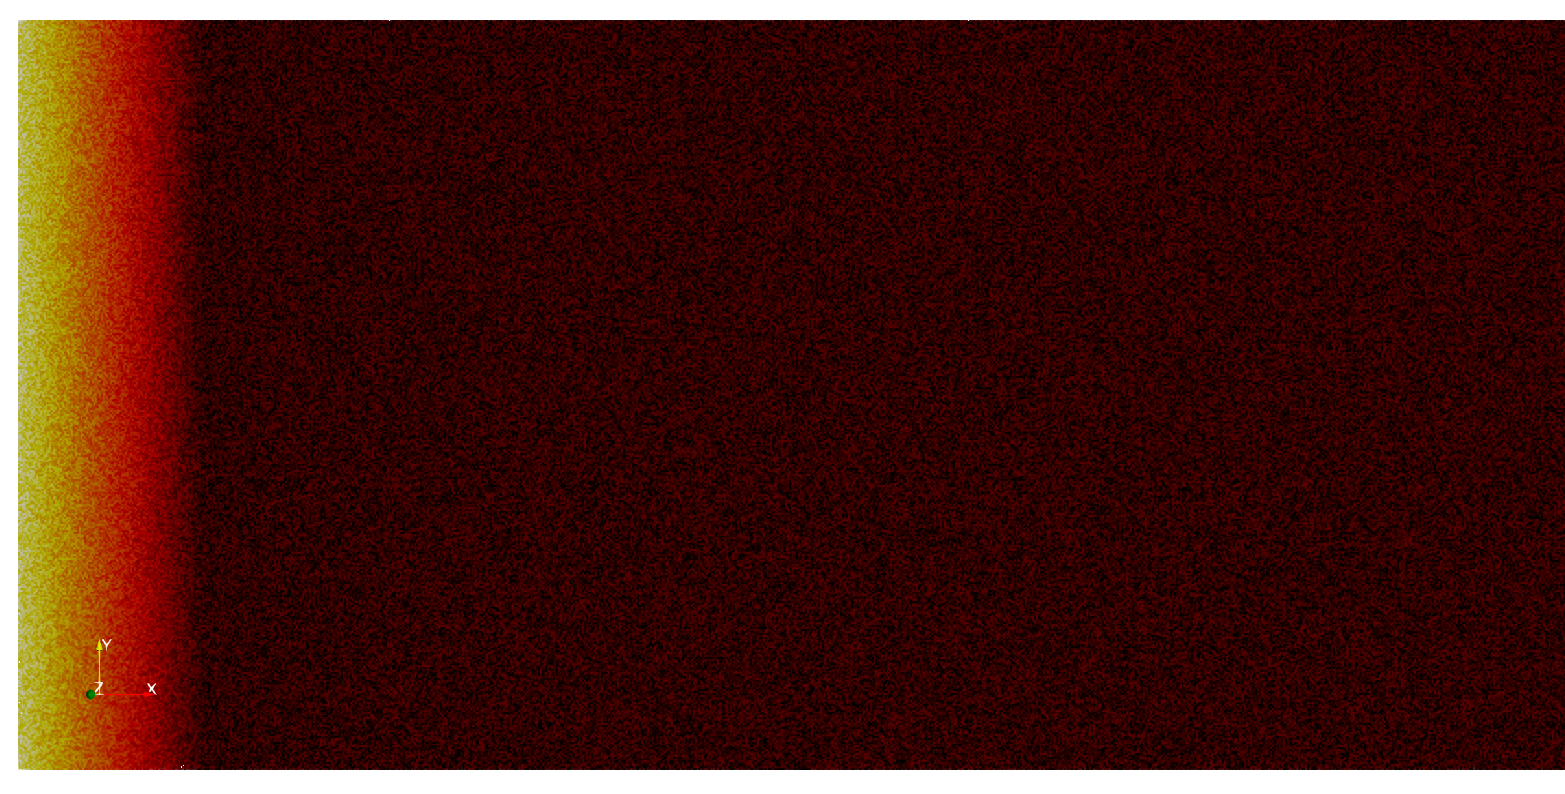
\includegraphics[width=0.8\textwidth]{figs/ignition/randgrad.png}
\caption{Gradient ignition method with randomized temperature distribution throughout domain, seen on left side of domain, at t = 0 s}
\label{fig:gradrand}
\end{figure}%
\noindent This was chosen as it is 20\% of the maximum initial ignition temperature, and should provide enough randomization to instantiate detonation cells. The randomization of temperature from +0 K to +240 K is uniform and not Gaussian in distribution. With the randomization 





\section{Arrhenius Pre-exponential Factor}
\label{sec:a}

Now that an appropriate solver was selected, the solver settings needed to be dialed in. To start, some further testing was performed on the units of the pre-exponential factor for the Arrhenius equation in the \verb|reactions| file. Since the geometry, boundary, and initial conditions are all matched to the setup for the detonation tube in Towery\cite{towery1}, we will use the results there as a generic target to determine the order of magnitude of the exponent on the pre-exponential factor. The exponent was swept between \(10^{11}\) through \(10^{17}\). The results are seen in Figures \ref{fig:atestp}, \ref{fig:atestt}, and \ref{fig:atestu}. 

\begin{figure}
\centering
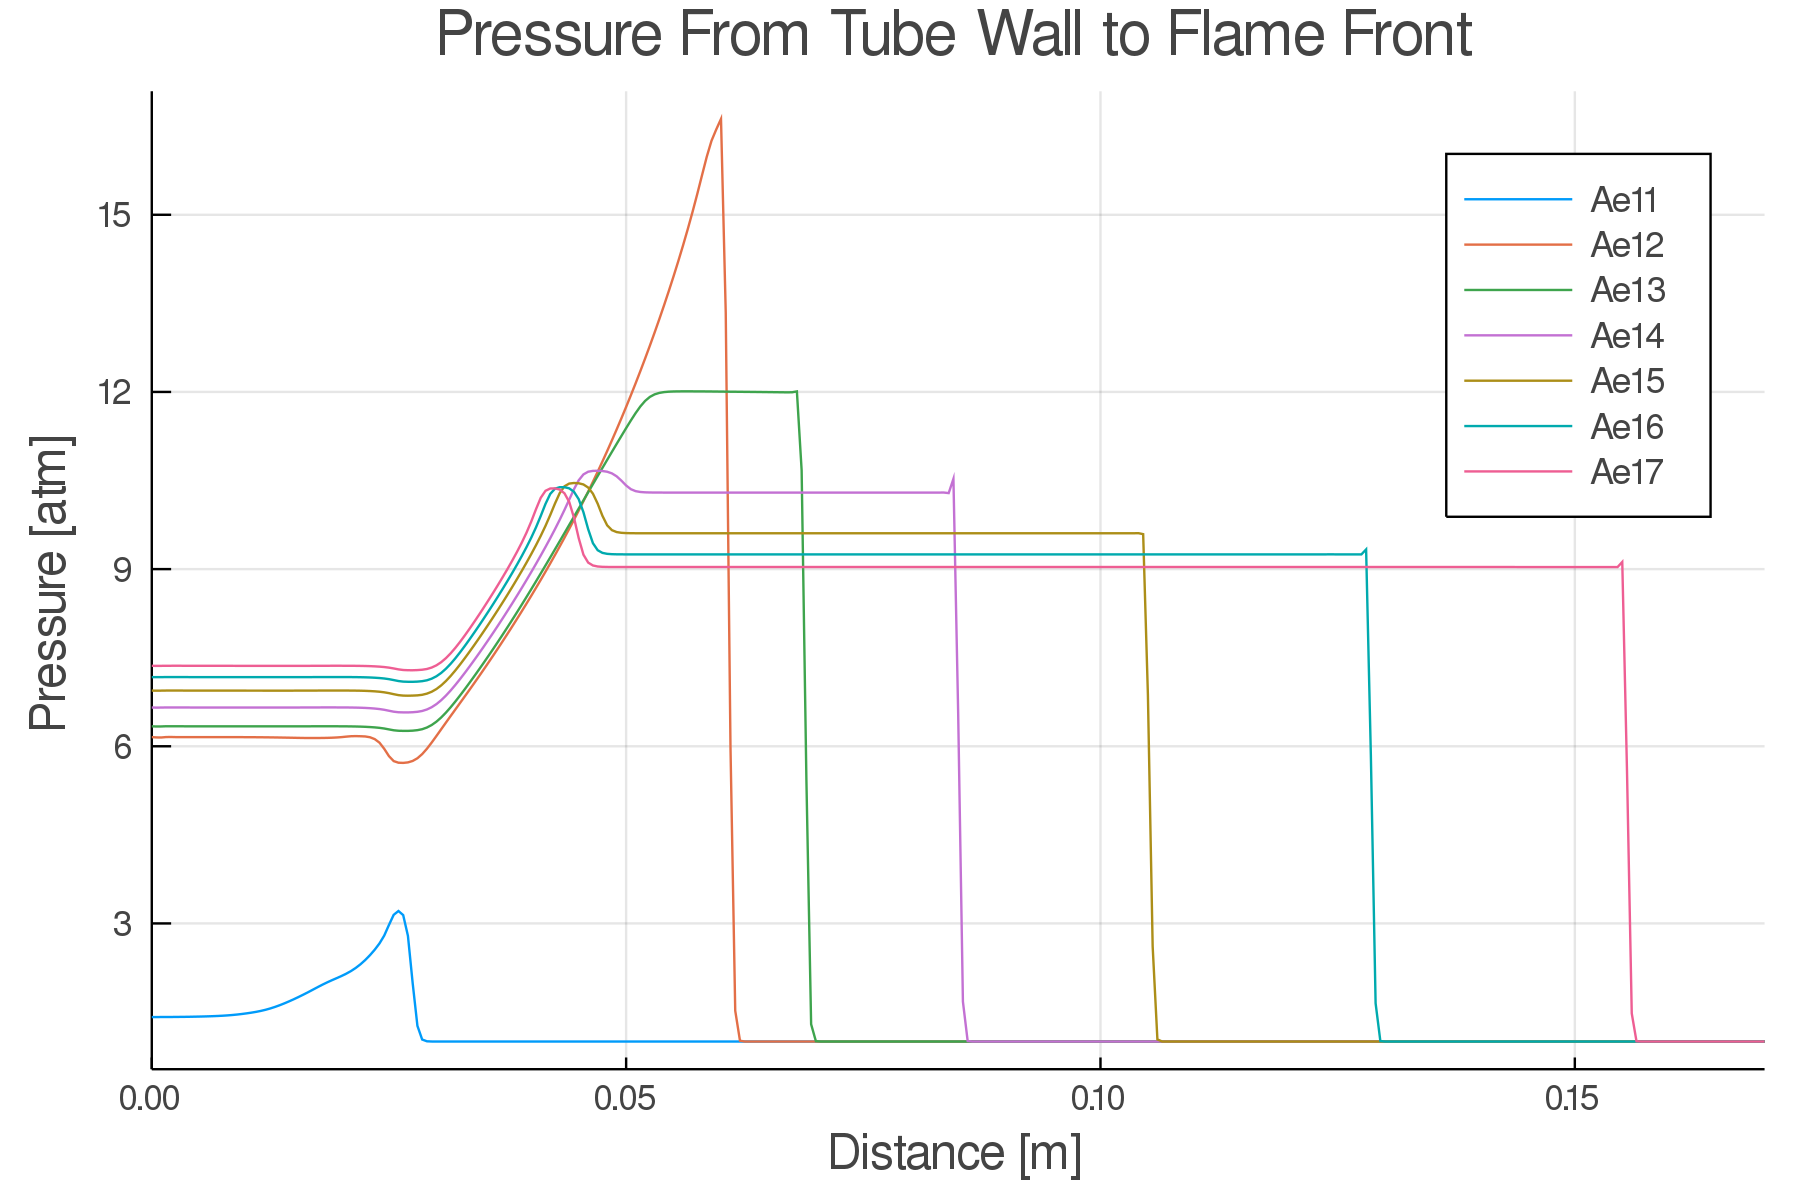
\includegraphics[width=0.85\linewidth]{./figs/Atest/p.png}
\caption{Pressure distribution in detonation tube for pre-exponential factor exponent sweep test}
\label{fig:atestp}
\end{figure}

\begin{figure}
\centering
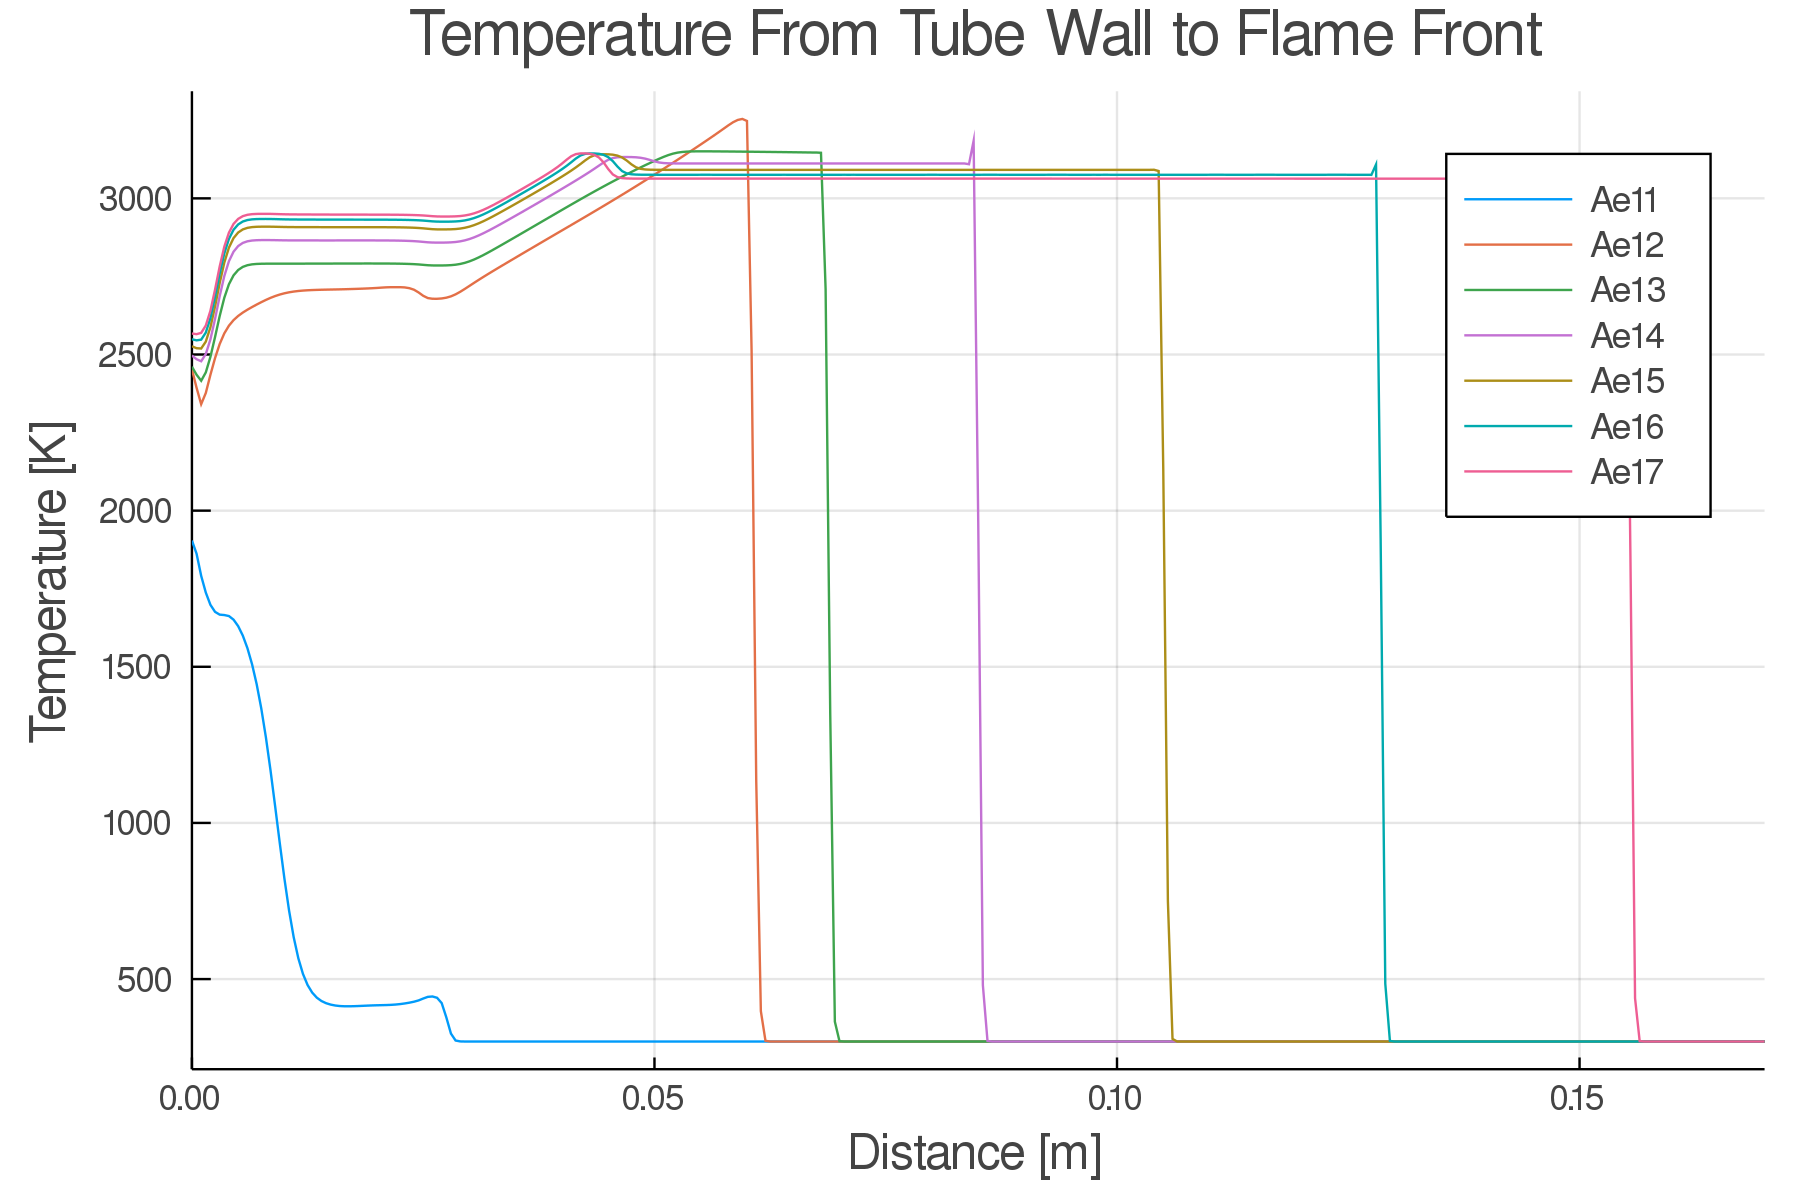
\includegraphics[width=0.85\linewidth]{./figs/Atest/t.png}
\caption{Temperature distribution in detonation tube for pre-exponential factor exponent sweep test}
\label{fig:atestt}
\end{figure}

\begin{figure}
\centering
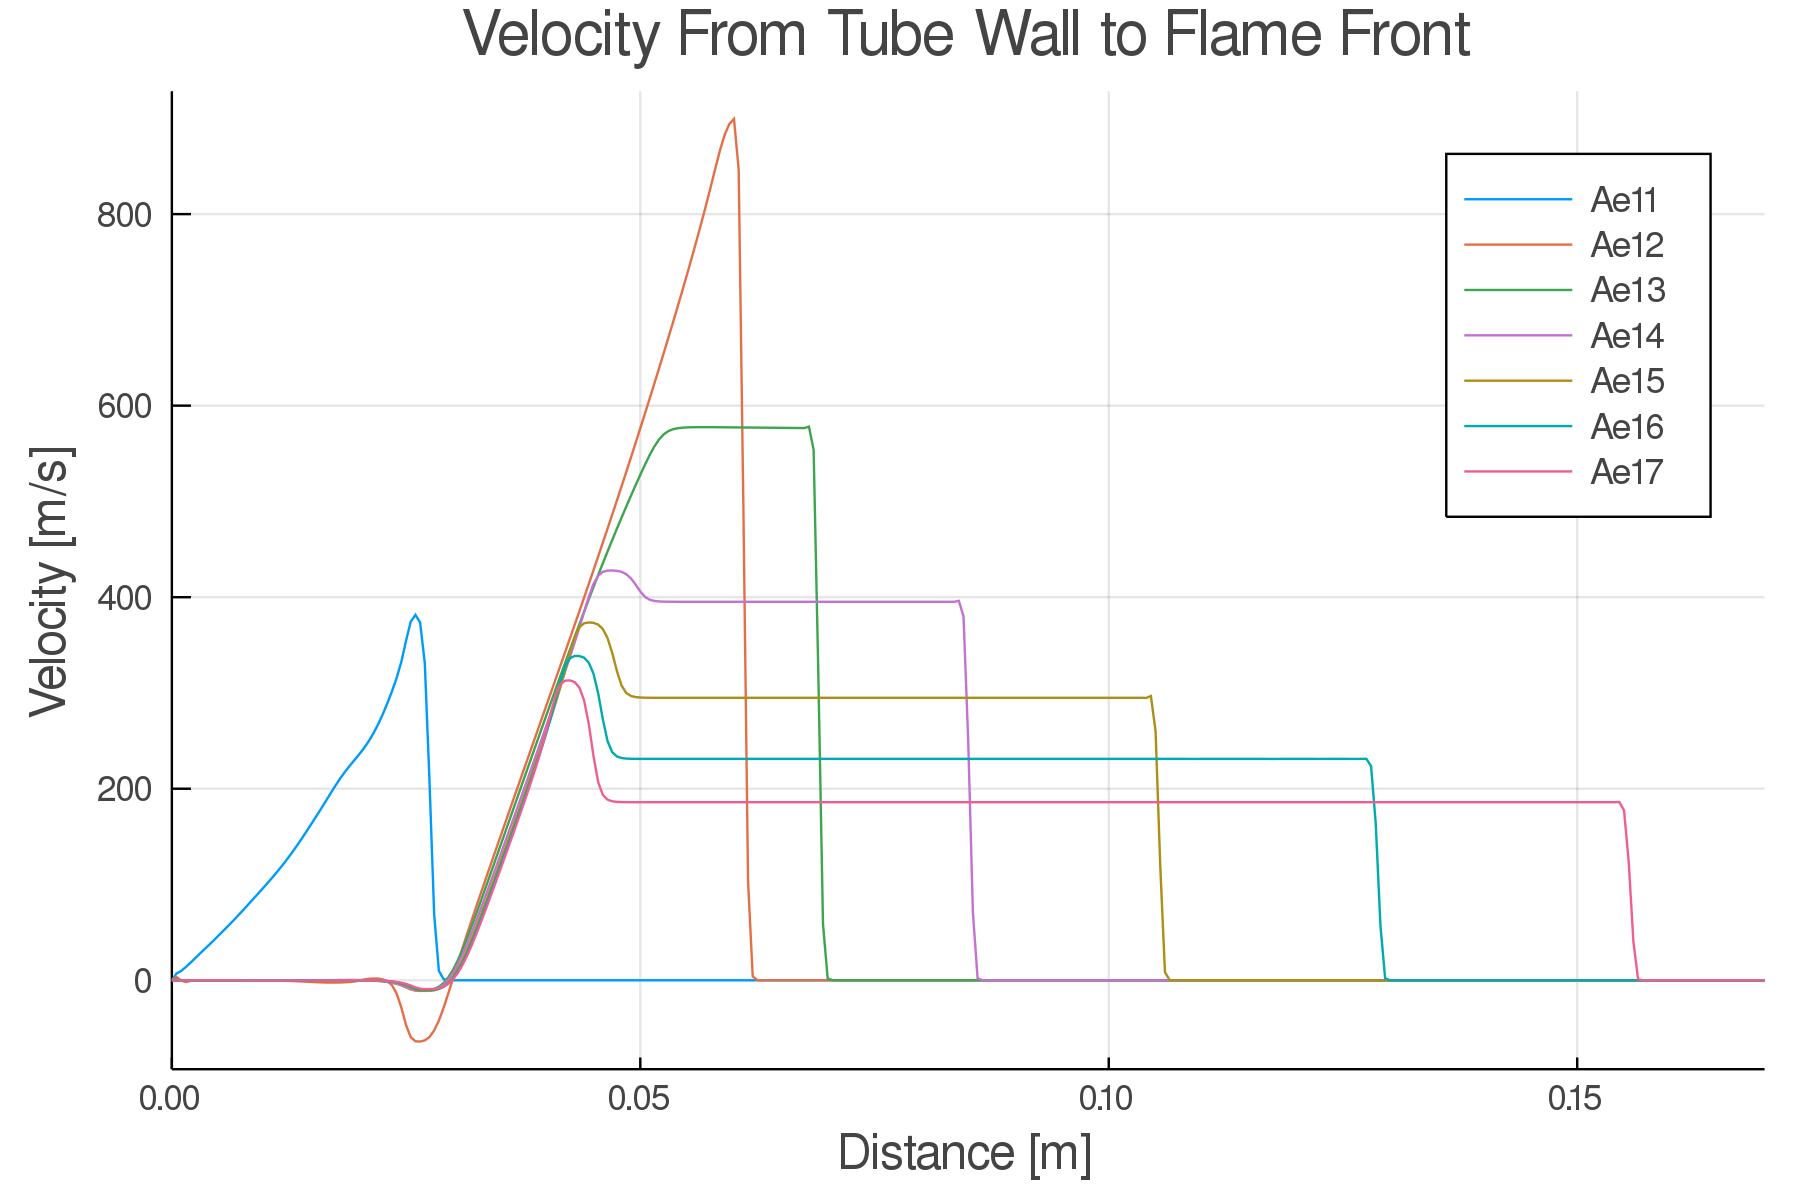
\includegraphics[width=0.85\linewidth]{./figs/Atest/u.png}
\caption{Velocity distribution in detonation tube for pre-exponential factor exponent sweep test}
\label{fig:atestu}
\end{figure}

From these figures, we can see the importance of having an accurate order of magnitude on the exponent for results. As the exponent was increased beyond the power of 12, plateaus emerge in the results for all thermodynamic variables. Under the power of 12, there is a large jump in solution, and a transition from between detonation states, seen in Figure \ref{fig:pjump}. The differences in these states is due to the coupling of the shockwave and the reactions (flame). The grouping of plots with higher pressure values have the reactions coupled with the shock, and the smaller pressure value grouping has the reaction occurring more slowly and trailing behind the shock. This is more evident in Figures \ref{fig:atestrp} and \ref{fig:atestrt} where we see that there is still a shockwave present in the ``lower'' group, but it is clear by Figure \ref{fig:atestrt} that the reaction process is happening much later than the shockwave instead right at the shock front. Thus presence of a shockwave in this scenario is not due to the sustained reaction, and was triggered by high pressure (and temperature) region used to initialize detonations in the simulation. 

\begin{figure}
\centering
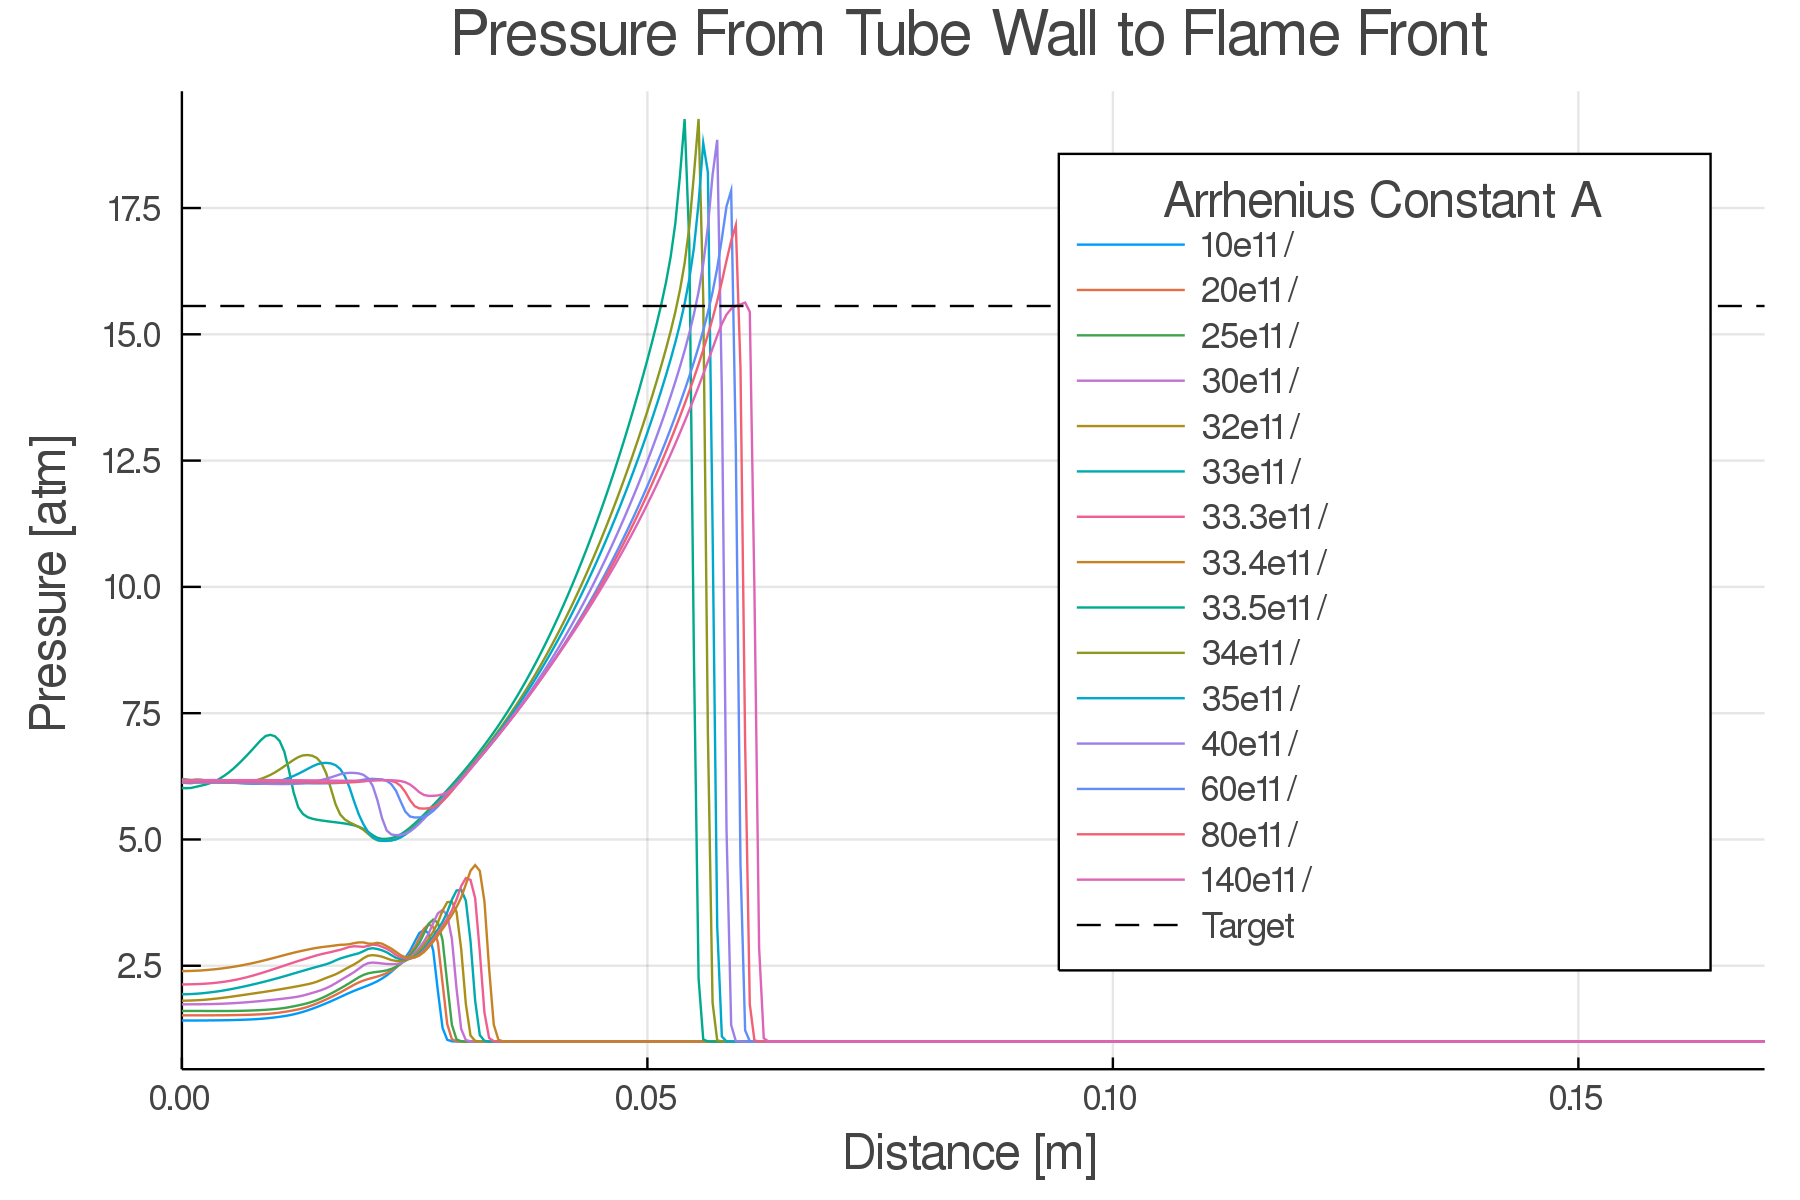
\includegraphics[width=0.85\linewidth]{./figs/Atest_refined/p_large.png}
\caption{Pressure distribution in detonation tube for expanded and refined pre-exponential factor exponent sweep test, showing detonation shock-reaction coupling transition. See Figures \ref{fig:atestrp} and r\ref{fig:atestrt} for a filtered version.}
\label{fig:pjump}
\end{figure}


The exponent in this region was explored further since plateaus in thermodynamic properties values are not physical for real-world detonations. Note that the velocity plotted in Figure \ref{fig:atestu} is a fluid velocity, not a wave velocity. When instead we swept over a smaller interval, with the Chapman-Jouguet (CJ) targets from Towery\cite{towery1} plotted, we can see that there is a very abrupt transition in detonation stability (Figures \ref{fig:atestrp} and \ref{fig:atestrt}). 

\begin{figure}
\centering
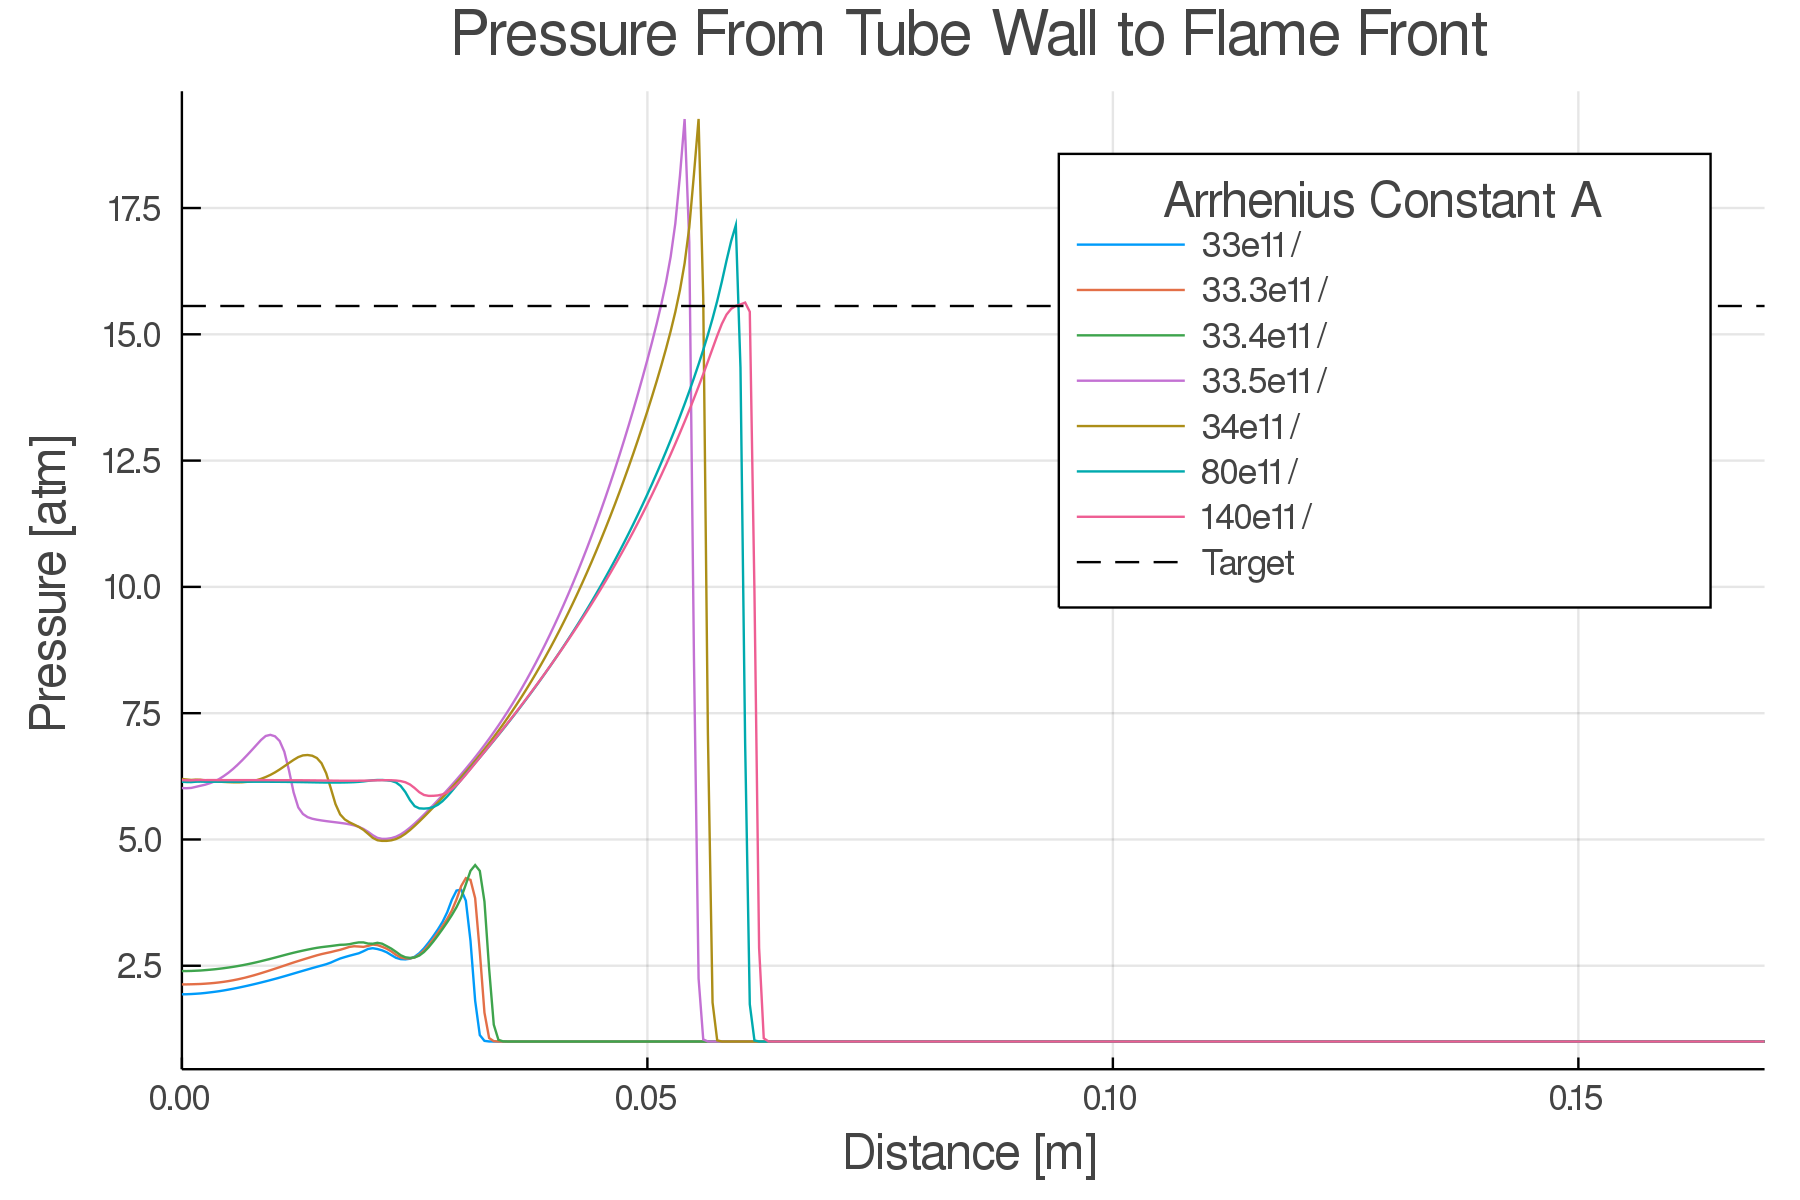
\includegraphics[width=0.85\linewidth]{./figs/Atest_refined/p.png}
\caption{Pressure distribution in detonation tube for refined pre-exponential factor exponent sweep test, filtered from Figure \ref{fig:pjump} and refined from Figure \ref{fig:atestp}}
\label{fig:atestrp}
\end{figure}

\begin{figure}
\centering
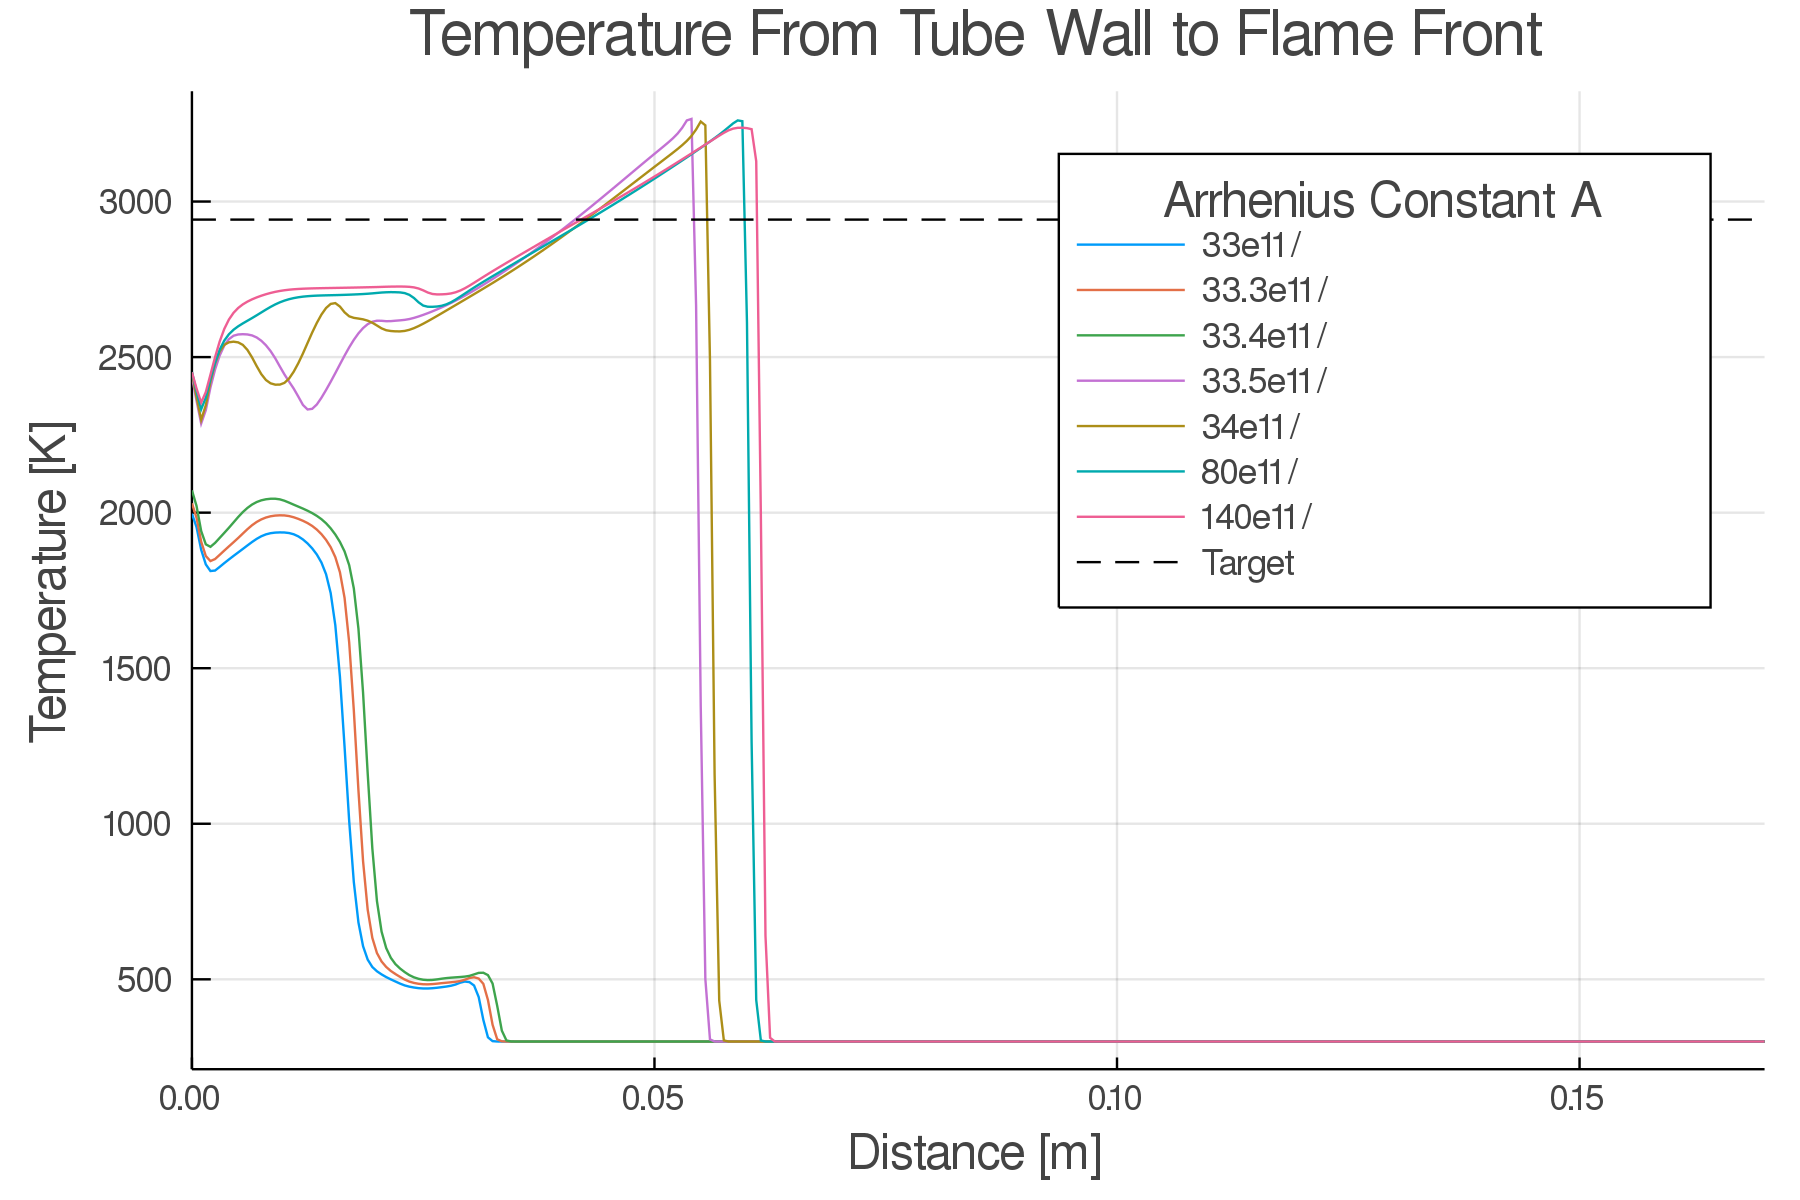
\includegraphics[width=0.85\linewidth]{./figs/Atest_refined/t.png}
\caption{Temperature distribution in detonation tube for refined pre-exponential factor exponent sweep test, refined from Figure \ref{fig:atestt}}
\label{fig:atestrt}
\end{figure}

With these tests, \(10^{13}\) was selected as an appropriate order of magnitude as it not only agreed with the results seen in Towery\cite{towery1}, but also with the value given for a single-step hydrogen-oxygen detonation in other published works\cite{hashemi}. 




\section{Time Step Variation}
One of the important tests was to determine how large the time step of the simulation could be taken. In OpenFOAM, one has several options for how the time step should be selected. By default, time steps are fixed, and set within \verb|controlDict|. Setting different values for how large the time step should be will affect the stability and solution of the simulation. Larger time steps will be more unstable, increasing the Courant number and sometimes leading towards the inability for solutions at a time step to converge. If we consider a fluid particle, the faster it moves, the more distance it can cover in a unit of time. If it is moving very quickly, large time steps mean this fluid particle could have traversed very far, leading to uncertainty in the solution. In a more general sense, we consider information and how it progresses throughout the gridded domain. For Courant numbers larger than one, the fluid is moving through more than one grid point per time step, and this is very difficult for the time integrators solving the flow equations to assess accurately. The logical choice would be to always select a very small time step to ensure a more stable and accurate solution. However, with decreased time step intervals comes increased computational cost, as the computer must solve the fluid equations much more often to arrive at a specific point in time. Instead, a smarter approach can be taken, where the time step is allowed to vary based on the Courant number. 

Inside \verb|controlDict| for \verb|rhoReactingCentralFoam|, we can set a maximum for both the typically-used fluid velocity Central Courant number as well as the acoustic (wave speed) Courant number. Each iteration, the solver will check the value of both these Courant numbers, and decrease the time step accordingly if the Courant number maximum is exceeded. In an effort to best determine how large the Courant number and therefore the time step can be, the maximum Courant number was set and swept across for various values. For these tests, a domain size of \( (x,y,z) = (0.5,0.04,0.04) \) meters was used with a 5000-3-3 mesh. This is pseudo-one-dimensional setup. Several maximum Courant (CFL) numbers were swept across, and the results at \(3\times 10^{ - 5}\)s are plotted in Figures \ref{fig:cflp}, \ref{fig:cflt}, and \ref{fig:cflu}. Note that the notation used in the plot omits the decimal point for the maximum CFL number, so \verb|5000_3_3_005| represents a 5000-3-3 mesh with a maximum CFL of 0.05. 

\begin{figure}[]
    \centering
    \begin{subfigure}[]{\textwidth}
    \centering
    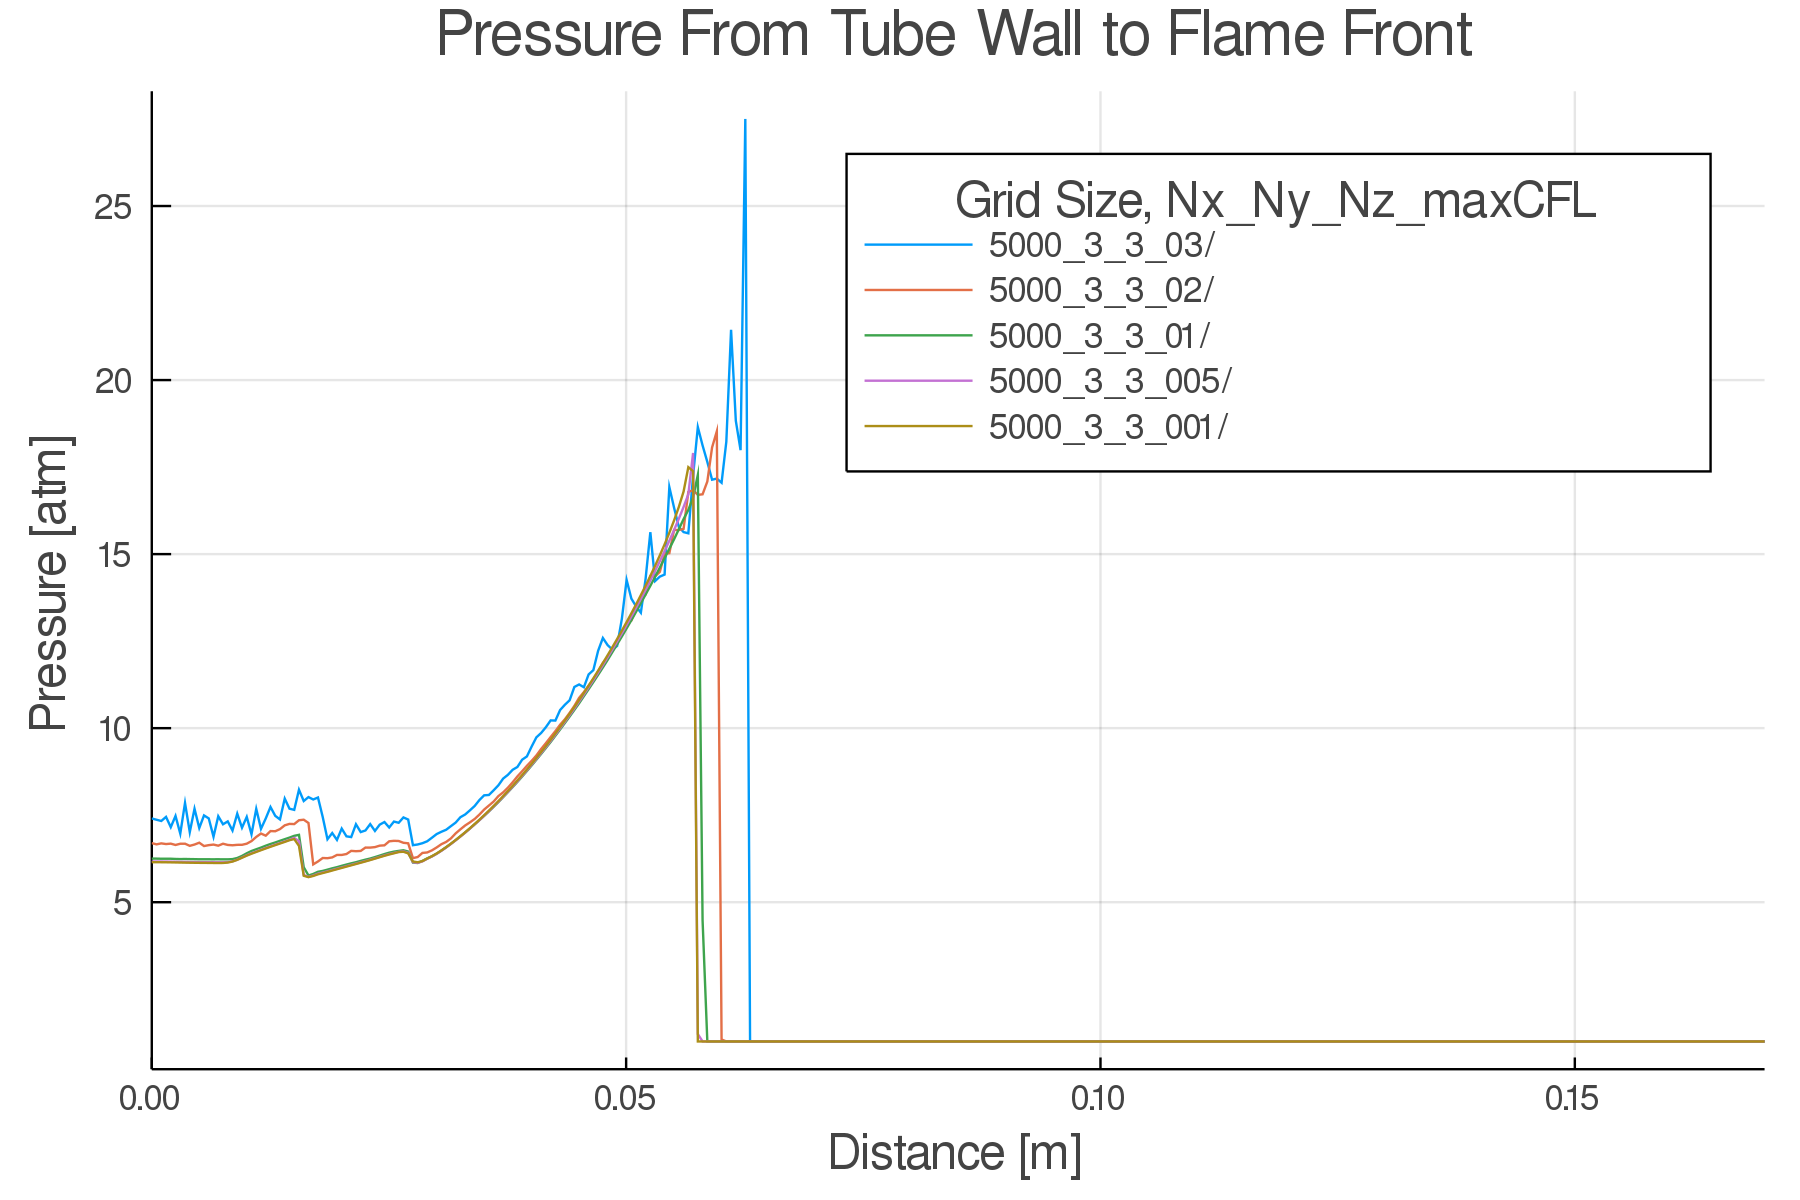
\includegraphics[width=\linewidth]{figs/cfl_test/p.png}
    \caption{Pressure distribution}
    \label{fig:cflp}
    \end{subfigure}

    \begin{subfigure}[]{\textwidth}
    \centering
    \includegraphics[width=\linewidth]{figs/cfl_test/t.png}
    \caption{Temperature distribution}
    \label{fig:cflt}
    \end{subfigure}
\end{figure}
\begin{figure}\ContinuedFloat
    \begin{subfigure}[]{\textwidth}
    \centering
    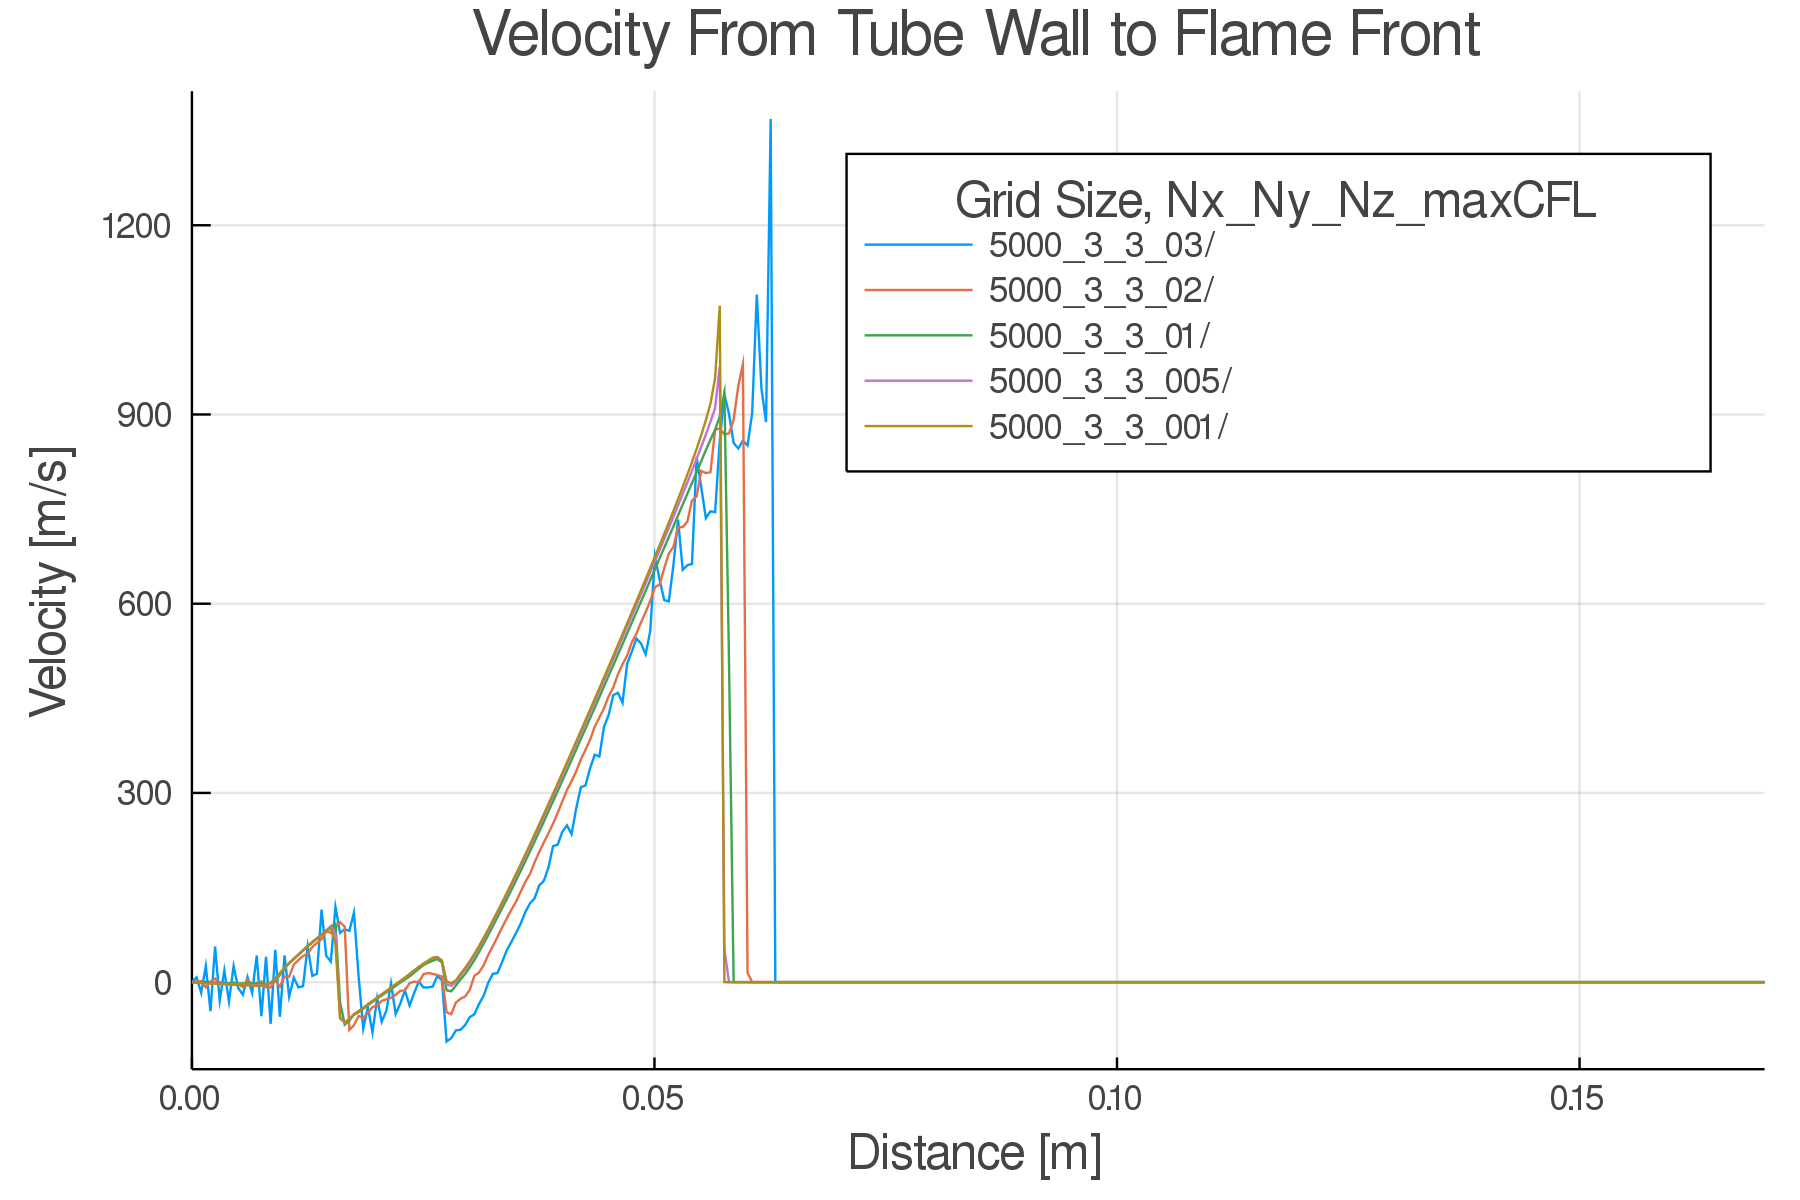
\includegraphics[width=\linewidth]{figs/cfl_test/u.png}
    \caption{Fluid velocity distribution}
    \label{fig:cflu}
    \end{subfigure}
    \caption{Max CFL sweep test}
    \label{fig:maxcfl}
\end{figure}



From Figures \ref{fig:cflp}, \ref{fig:cflt}, and \ref{fig:cflu}, it is seen that there is decreased noise in the solution as well as convergence as the time step and therefore maximum CFL is decreased. More evident in the temperature plot \ref{fig:cflt}, noise and instability is especially clear in the detonation simulations with maximum CFLs of 0.2 and 0.3. The CFL of 0.1 was decided to be acceptably converged due to a small comparative error, seen in Table \ref{tab:cflerror}. 
\begin{table}[]
\centering
\caption{Max CFL errors compared to CFL = 0.01}
\label{tab:cflerror}
\begin{tabular}{cccc}
Max CFL & Pressure Error (\%) & Temperature Error (\%) & Velocity Error (\%) \\ \hline
0.3 & 57.18 & 19.54 & 27.62 \\ 
0.2 & 5.89 & 8.72 & 8.66 \\
0.1 & 1.28 & 2.71 & 12.92 \\
0.05 & 2.34 & 1.29 & 8.96 \\
0.01 & 0 & 0 & 0 \\
\end{tabular}
\end{table}% 
\noindent Note that while the CFL of 0.2 has a smaller velocity error than the CFL of 0.1, it is a much noisier and unstable solution, so the values themselves have further uncertainty. The selection of a maximum CFL of 0.1  for detonations in OpenFOAM also matches with the work done by Ajaero\cite{ajaero}. 

Higher CFL numbers of 0.4 to 0.8 were also attempted. These were unsuccessful as the solution was extremely unstable at these CFLs. Typically, high CFL numbers cause more ringing in the solution as seen in Figure \ref{fig:maxcfl} for the CFL of 0.3. However, it is seen in this research as well as supporting reacting flow work \cite{ajaero} that lower CFL numbers are required for solution convergence. 

\section{Static Mesh Variation}
\label{sec:staticvar}
In order to determine the performance gains, accuracy, and other comparative parameters between mesh resolutions, baseline meshes must be created. These meshes must not change adaptively in the simulation in order to provide clear comparisons. Additionally, the static meshes themselves should be compared with each other to determine when mesh convergence occurs. Once a mesh resolution is determined, the AMR parameters can be tuned in an attempt to match the static mesh resolution in the small region surrounding the detonation wave. 


\subsection{One-dimensional}
The first set of static mesh comparisons performed is between one-dimensional detonation tube simulations, seen in Figure \ref{fig:1dstatic}. These meshes only have resolution along the direction of the tube, which allows for capturing the detonation wave as simply as possible. However,  one-dimensional detonation tube simulations are not optimal for generic detonation modeling as the cellular detonation structure seen in experimental detonation modeling cannot be captured with a single dimension. The cellular detonation cells can be used to infer velocity and compare numerical simulation with experiments, so one-dimensional detonations must utilize other methods to compare with experiments or just be utilized for tuning numerical methods themselves. 

\begin{figure}[]
    \centering
    \begin{subfigure}[]{\textwidth}
        \centering
        \includegraphics[width=\textwidth]{./figs/static1d/p.png}
        \caption{Pressure plot}
    \end{subfigure}

    \begin{subfigure}[]{\textwidth}
        \centering
        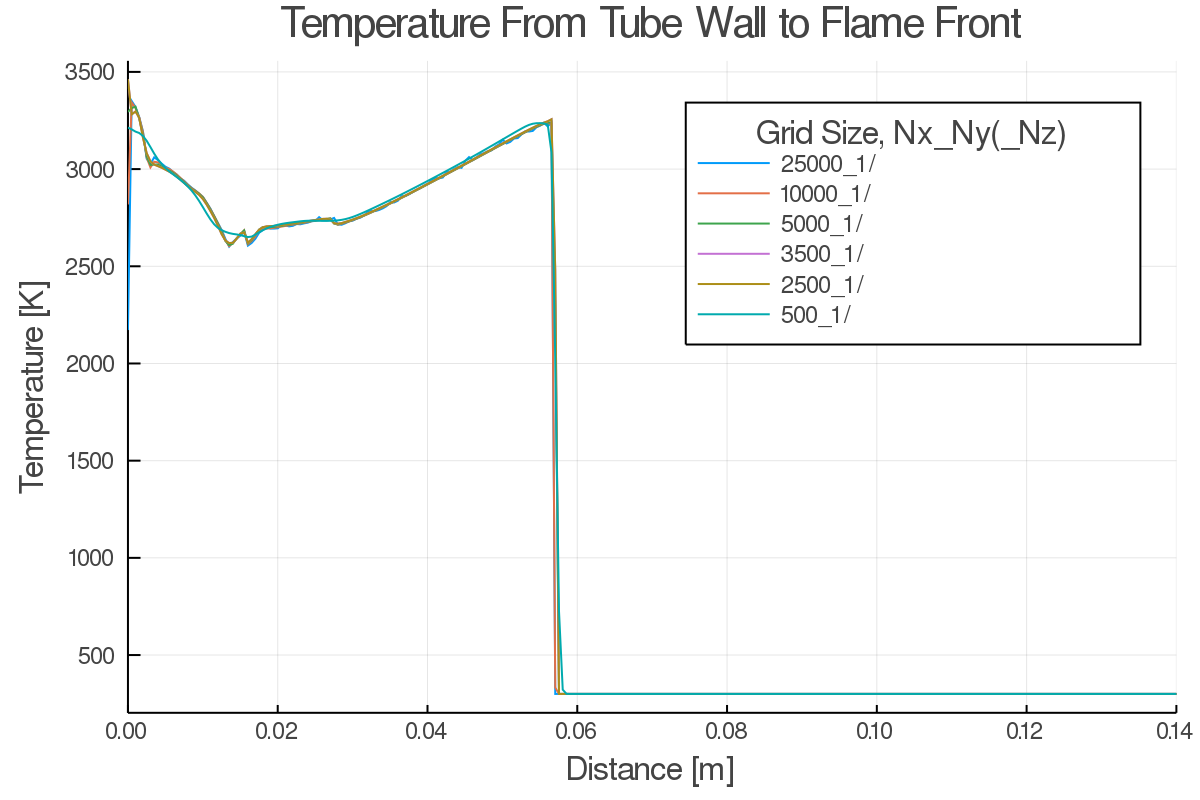
\includegraphics[width=\textwidth]{./figs/static1d/t.png}
        \caption{Temperature plot}
    \end{subfigure}

\end{figure}
\begin{figure} \ContinuedFloat
    
    \begin{subfigure}[]{\textwidth}
        \centering
        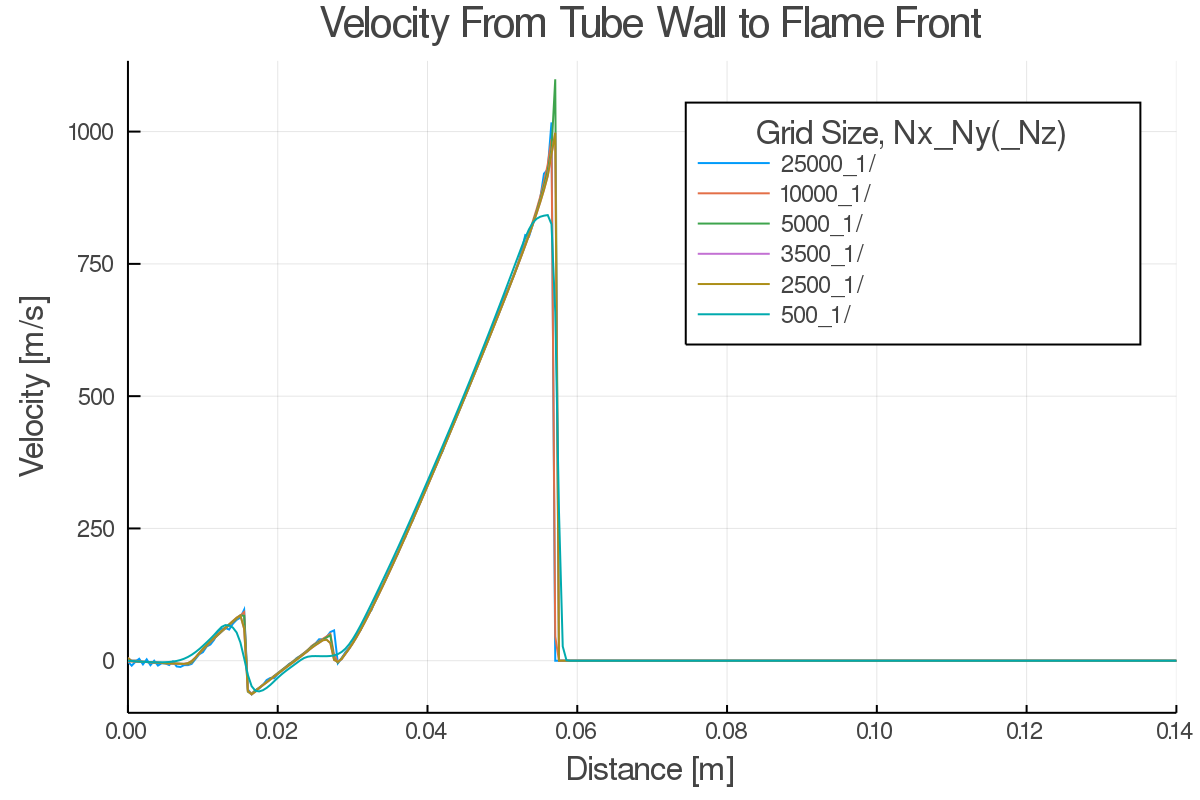
\includegraphics[width=\textwidth]{./figs/static1d/u.png}
        \caption{Fluid Velocity plot}
    \end{subfigure}

    \caption{One-dimensional static meshes used in detonation tube simulations}
    \label{fig:1dstatic}
\end{figure}

Various static one-dimensional meshes were compared and can be seen in Figure \ref{fig:1dstatic}. These one-dimensional static meshes are actually twice as long, as initially the detonation simulations were performed using a mesh that was twice as long. This long mesh was unnecessarily large and computationally expensive. The mesh partition values written in the figure are divided in half to match the meshes and convention used in subsequent analysis runs. We see that the 500-1-1 mesh has not converged yet to a solution, and that the 2500-1-1 mesh has converged. After this point, the difference between the meshes lies in their ability to capture finer flow effects such as detonation cells (not possible in one dimension), the transition from a singular detonation front to the combination of multiple smaller detonation fronts (also not possible in one dimension), and the increase in magnitude of the von Neumann pressure wave spike. The von Neumann spike comes from ZND detonation model theory, where Zel'dovich\cite{zeldovich}, von Neumann\cite{neumann}, and Doring\cite{doring} independently published research on a detonation model theory that utilizes an infinitesimally thin shock wave. Knowing that the spike is what changes within the converged mesh simulations allows for intelligent choices upon what sorts of AMR and static resolutions to choose both in research and engineering design. If an individual is designing a part that can withstand very fast high pressure fluctuations, then resolving the mesh up until the von Neumann spike appears will be sufficient for their design purposes. Otherwise, further mesh resolution is required in order to resolve the extremely thin pressure spike shock region. In regards to AMR, this translates to either further refinement around the spike region or just focusing refinement on the detonation wave and following region as a whole in order to resolve turbulence details or fluctuations in the field from randomization and reflected shocks. 


\subsection{Two-dimensional}
In addition to the static and dynamic one-dimensional detonation tube simulations performed, two-dimensional simulations were also run. These can be seen in Figure \ref{fig:2dstatic}. 
\begin{figure}[]
    \centering
    \begin{subfigure}[]{\textwidth}
        \centering
        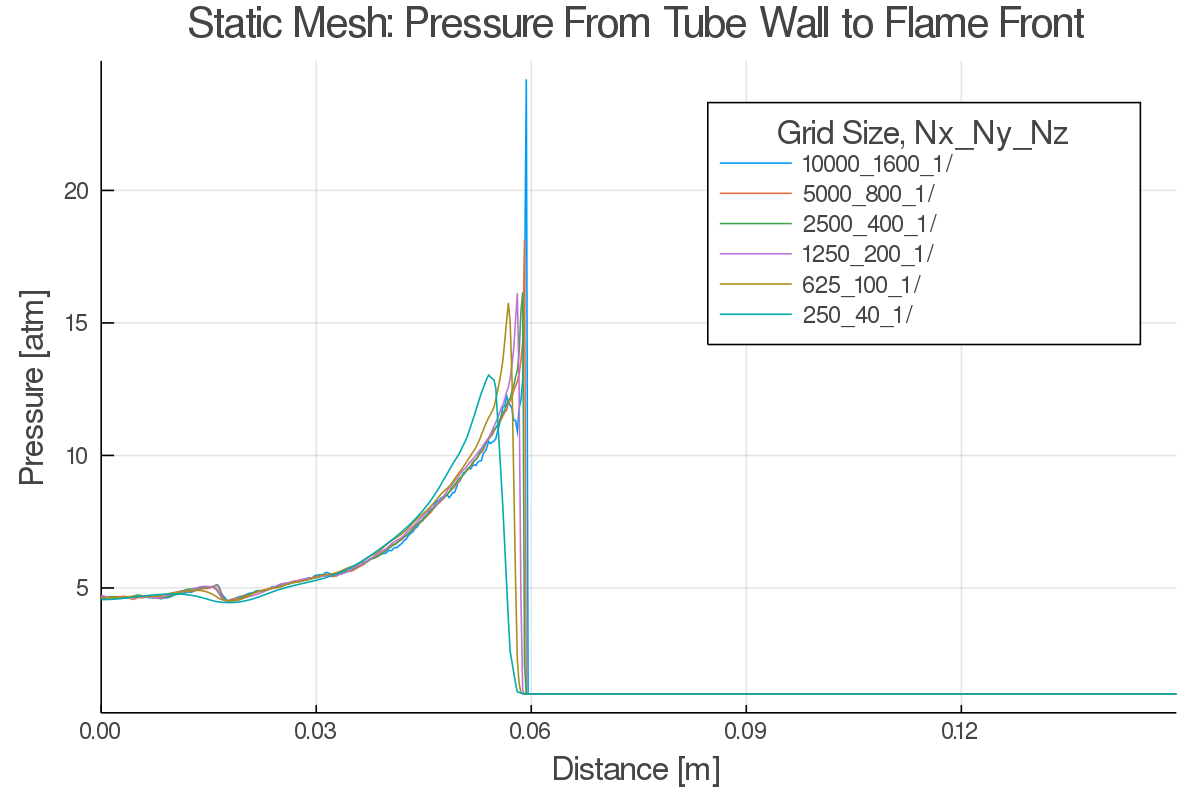
\includegraphics[width=\textwidth]{./figs/static2d/p.png}
        \caption{Pressure plot}
    \end{subfigure}

    \begin{subfigure}[]{\textwidth}
        \centering
        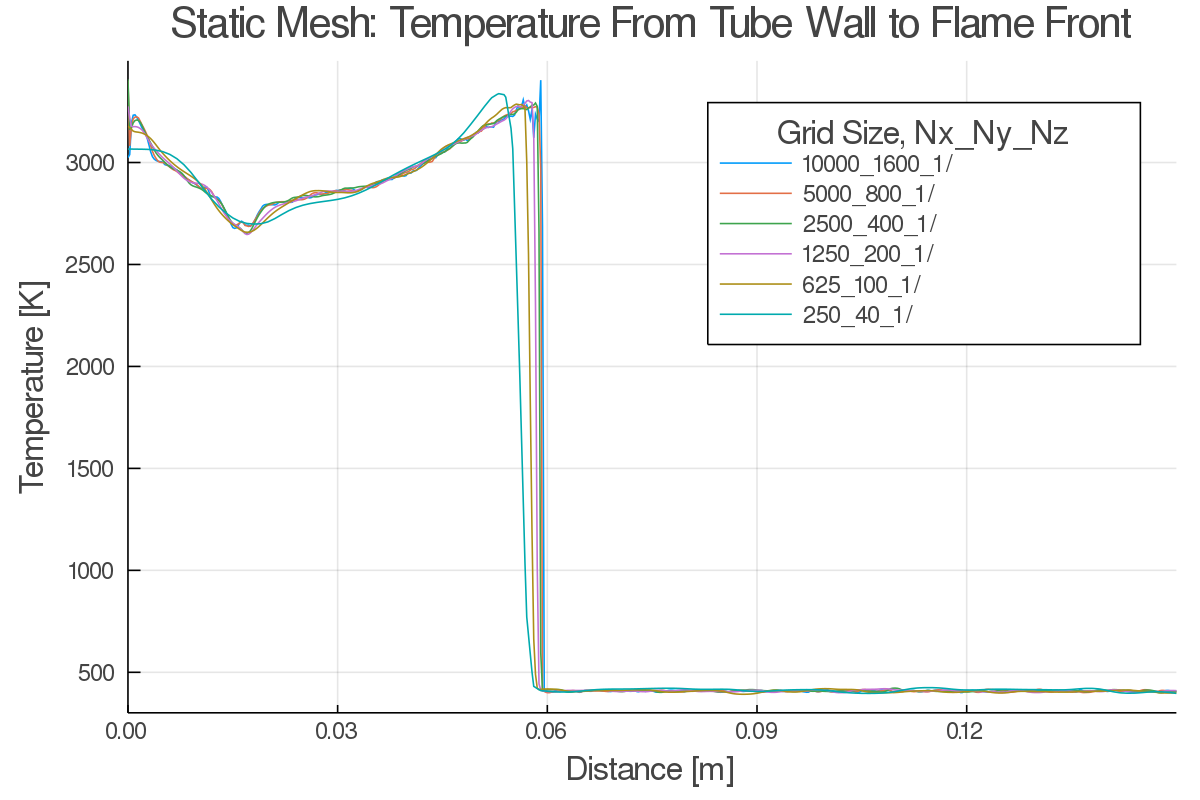
\includegraphics[width=\textwidth]{./figs/static2d/t.png}
        \caption{Temperature plot}
    \end{subfigure}

\end{figure}
\begin{figure} \ContinuedFloat
    
    \begin{subfigure}[]{0.95\textwidth}
        \centering
        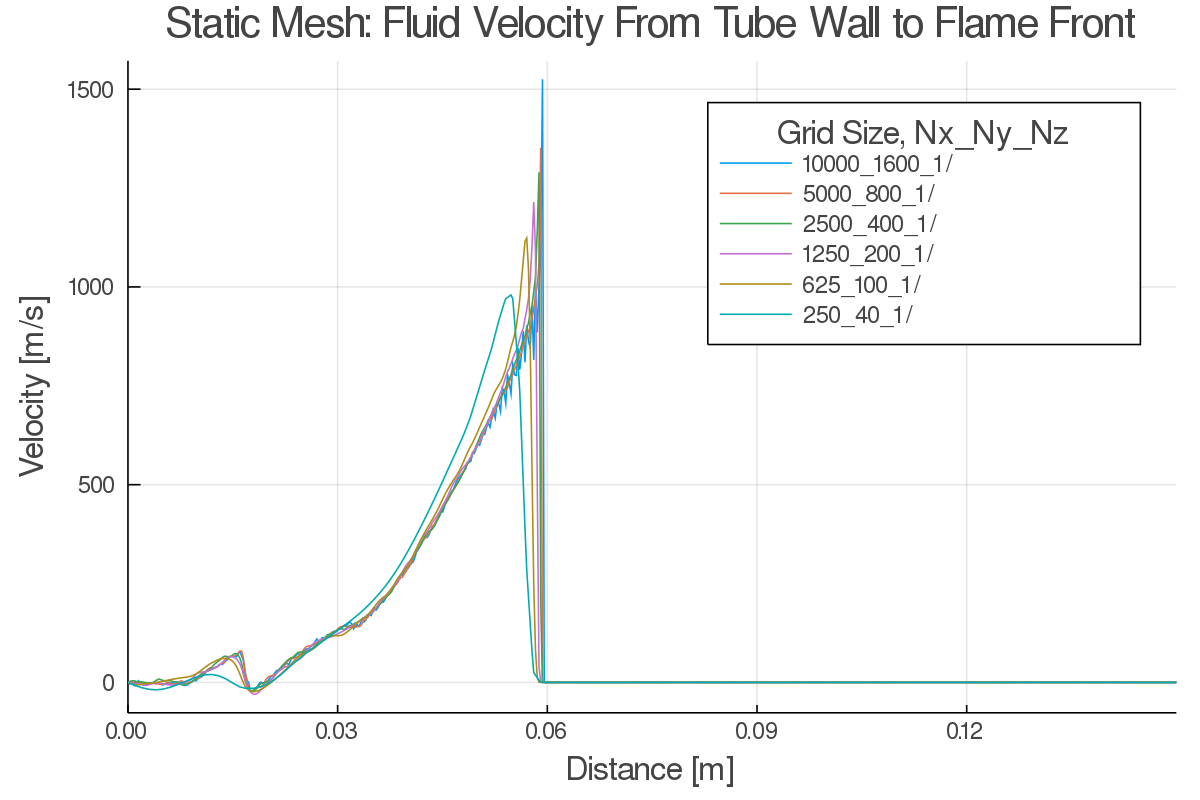
\includegraphics[width=\textwidth]{./figs/static2d/u.png}
        \caption{Fluid velocity plot}
    \end{subfigure}

    \begin{subfigure}[]{0.95\textwidth}
        \centering
        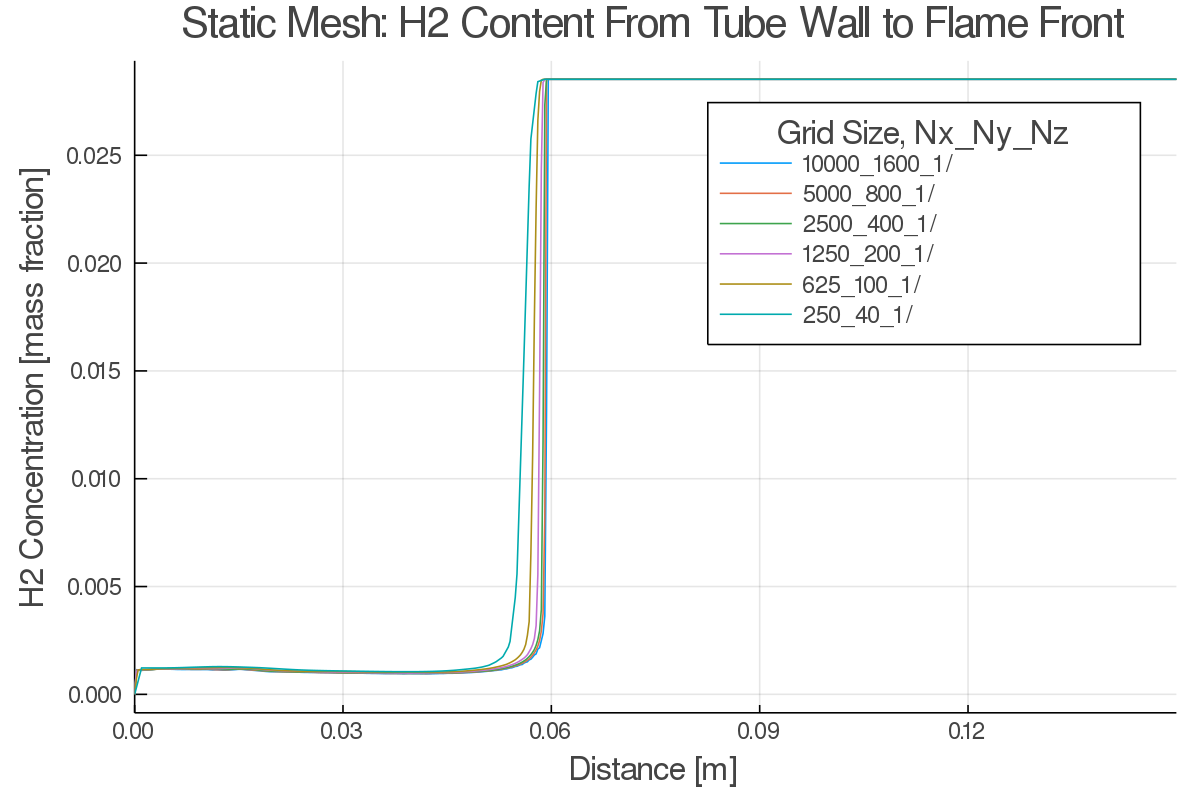
\includegraphics[width=\textwidth]{./figs/static2d/y.png}
        \caption{H\(_2\) mass fraction plot}
    \end{subfigure}

    \caption{Two-dimensional static meshes used in detonation tube simulations}
    \label{fig:2dstatic}
\end{figure}% 
For two-dimensional simulations, the mesh was kept square. A smaller mesh resolution than the one-dimensional simulations were used due to computational expense. The 10000-1600-1 mesh contains 16 million cells at a 25 micron physical resolution, and was computed across twenty 3.6 Ghz AMD Threadripper cores at a computational time of over 150 hours. Example surface plots for the static 2500-400-1 mesh are plotted in Figure \ref{fig:2dsurface}. 
\begin{figure}[]
    \centering
    \begin{subfigure}[]{\textwidth}
        \centering
        \includegraphics[width=\textwidth]{./figs/example_results/p.png}
        \caption{Pressure plot}
    \end{subfigure}

    \begin{subfigure}[]{\textwidth}
        \centering
        \includegraphics[width=\textwidth]{./figs/example_results/t.png}
        \caption{Temperature plot}
    \end{subfigure}

\end{figure}
\begin{figure} \ContinuedFloat
    
    \begin{subfigure}[]{\textwidth}
        \centering
        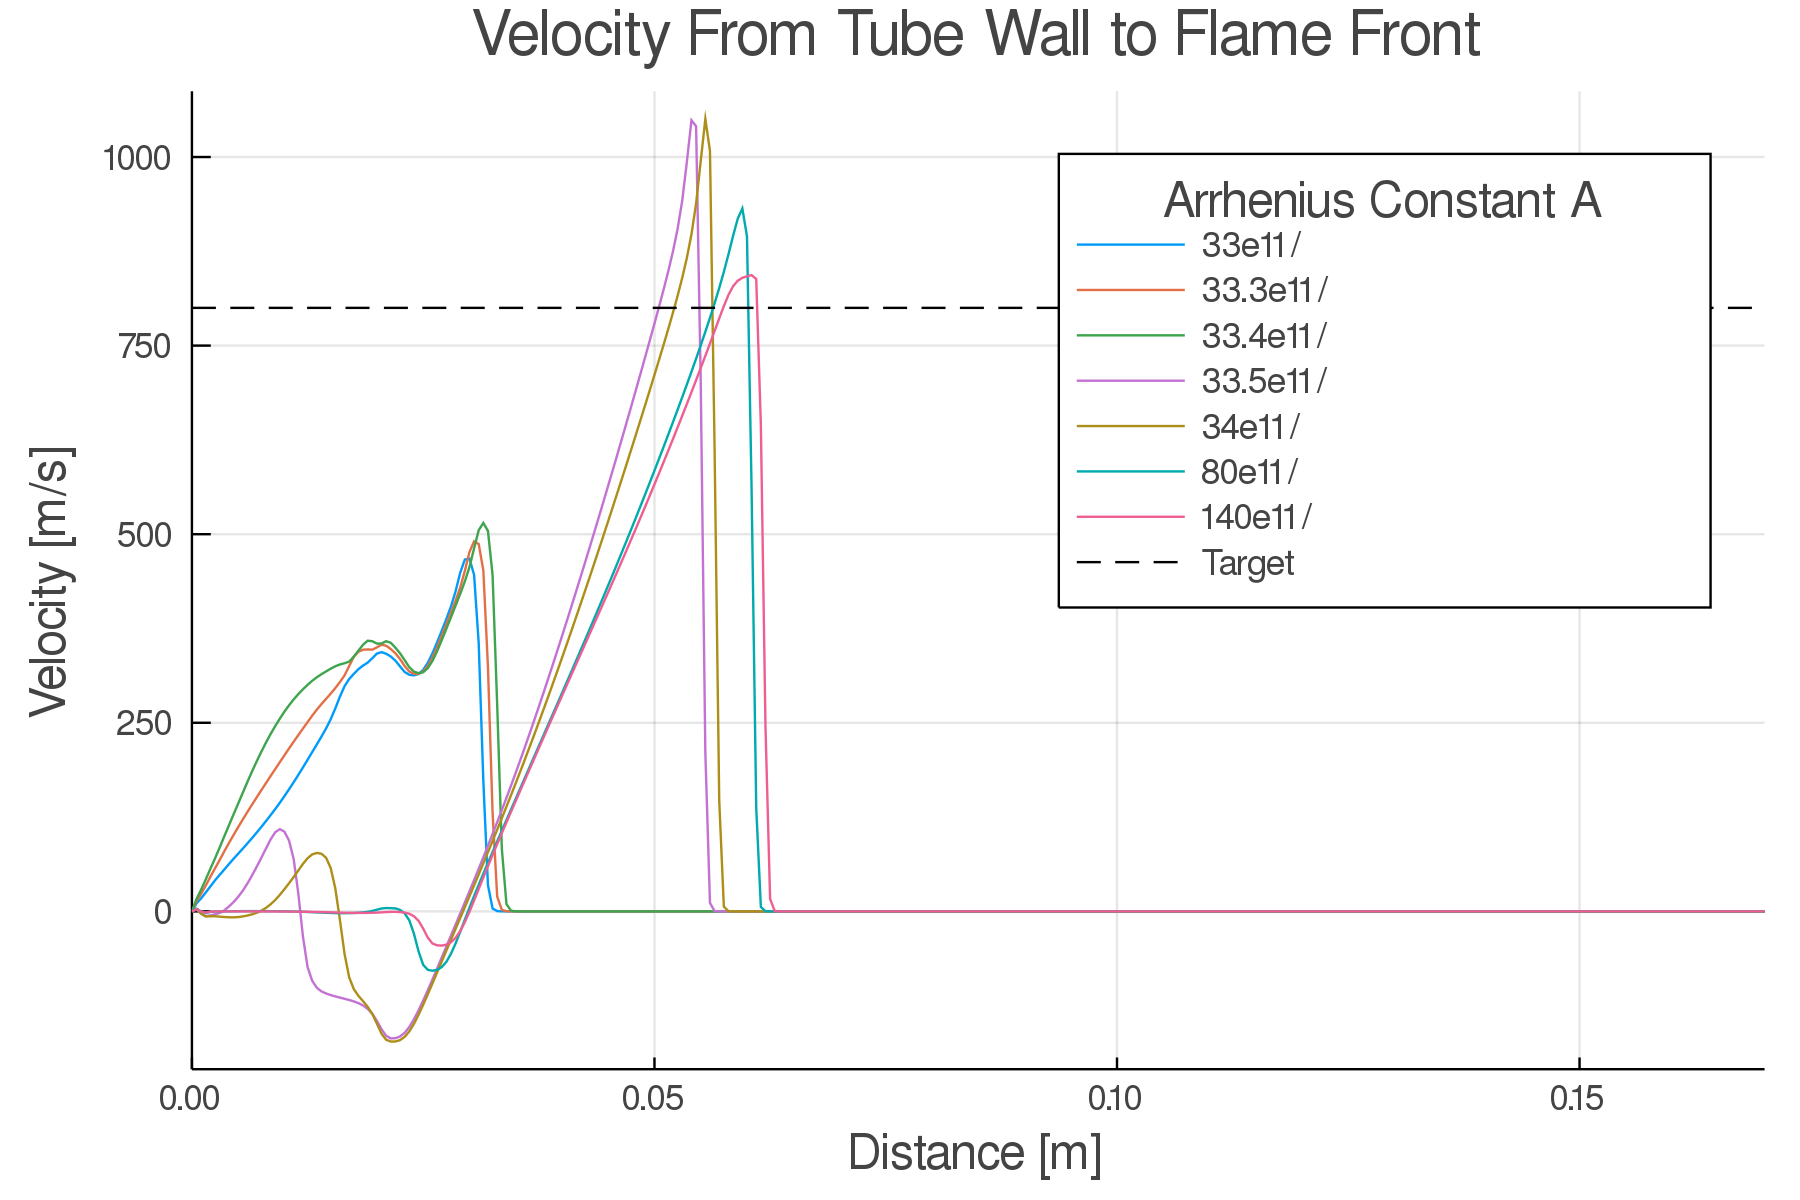
\includegraphics[width=\textwidth]{./figs/example_results/u.png}
        \caption{Fluid velocity magnitude plot}
    \end{subfigure}

    \begin{subfigure}[]{\textwidth}
        \centering
        \includegraphics[width=\textwidth]{./figs/example_results/rho.png}
        \caption{Density plot}
    \end{subfigure}

    \caption{Two-dimensional detonation wave surface plots for 2500-400-1 mesh at \(t = 3.45 \times 10^{ - 5} \) s}
    \label{fig:2dsurface}
\end{figure}% 
\noindent The plots seen in this figure represent the flow field results of a detonation wave traveling from the left wall to the right, at \(t = 3.45 \times 10^{ - 5} \) s. 





\section{Adaptive Mesh Refinement and Static Comparisons}
As mentioned in Section \ref{sec:staticvar}, the adaptive mesh refinement parameters can be tuned to try and match the fine static mesh resolutions in important areas. Detonation waves are very thin with extremely high pressures, temperatures, and velocities within this small region. This makes them an ideal candidate for adaptive meshing. 



\section{Sensitivities, efficiencies of AMR?}